
%\documentclass[oneside]{article}
\documentclass[11pt, a4paper]{article}
\usepackage{fontspec}
\usepackage[a4paper]{geometry}
\usepackage[export]{adjustbox}
\usepackage{graphicx}
%\usepackage[demo]{graphicx}
\usepackage{enumerate}
\usepackage{fancyhdr}
\usepackage{tocbibind}
\usepackage{lastpage}
\usepackage{tcolorbox}
\usepackage{amsmath}
\usepackage{xlop}
\usepackage{fancyhdr}
% \geometry{a4paper,margin=10mm,bindingoffset=20mm,heightrounded,}
\pagestyle{fancy}
%\fancyhf{}
%\rhead{}
%\lhead{Guides and tutorials}



%\usepackage[letterpaper, landscape, margin=2in]{geometry}

\usepackage[colorlinks=true]{hyperref}
\usepackage{setspace}
\usepackage[absolute]{textpos}
\setlength{\TPHorizModule}{1cm}
\setlength{\TPVertModule}{1cm}
\usepackage{xepersian}
\usepackage{titling}

\usepackage{lipsum}
\usepackage{scrextend}
\deffootnote[1.8em]{0pt}{1.6em}{\makebox[1.8em][l]{.\thefootnotemark}}
\newtheorem{theorem}{قضیه}
\newtheorem{corollary}{گزاره}
\newtheorem{lemma}{لم}
%%%%%%%%%%%%%%%%%%%%%%%%%%%%%%
%\usepackage{tikz}
%\usetikzlibrary{calc}
%\usetikzlibrary{decorations.pathmorphing}

%\usepackage{lipsum}% dummy text

\usepackage{color}
\definecolor{Darkblue}{rgb}{0,0,0.7}
\definecolor{pink}{rgb}{1,0.078,0.576}
\usepackage{hyperref}
\hypersetup{%
    pdfborder = {0 0 0},
    colorlinks,
    citecolor=red,
    filecolor=Darkblue,
    linkcolor=Darkblue,
    urlcolor=cyan!50!black!90
}

%\pagestyle{headings}

%%%%%%%%%%%%%%%%%%%%%%%%%%%%%%%%%
\settextfont[Scale=1.1]{B Nazanin}
\setlatintextfont{Times New Roman}
\defpersianfont\nastaliqfont{IranNastaliq}
\linespread{2.25}
\pagestyle{fancy}
\addtolength{\headheight}{\baselineskip}
\renewcommand{\sectionmark}[1]{\markboth{#1}{}}
%\renewcommand{\subsectionmark}[1]{\markright{#1}}
%\rhead{\leftmark\\\rightmark}

%\renewcommand{\headrulewidth}{0pt}
%\fancyhf{}
\newcommand*{\fancypagenumber}{%
\fancyfoot[C]{صفحه
\thepage
از
\pageref{LastPage}}
}
\fancypagenumber
\fancypagestyle{plain}{\fancypagenumber}
%\fancyhf{}
\newcommand{\logo}[1]{%
  \postauthor{%
  \end{tabular}\par\end{center}
  \begin{center}\includegraphics[scale=0.15]{#1}\end{center}
  \vskip0.5em}%
}
\logo{./pic/logo2}
\title{
 عنوان پروژه:
\\
\lr{Open Ran in 5G}
}

\author{\textsc{مژده کربلایی مطلب} % Author
\\{استاد راهنما: جناب آقای دکتر شاه منصوری}
%
\includegraphics[width=0.25\textwidth]{logo2}\\
%\\{دانشگاه صنعتی امیرکبیر-دانشکده ی برق}
}
%\address{}{\textbf{Amirkabir University of Technology -- Department of Electrical Engineering}}
%\logo{logo2}

% Definition of \maketitle
\makeatletter         
\def\@maketitle{
\raggedright

\includegraphics[width = 30mm]{./pic/logo1.png}\hspace{170 pt}

\includegraphics[width = 40mm]{./pic/logo3.png} \\[16ex] 
\begin{center}
{\Large \bfseries  \@title }\\ 
{\Large  \@author}\\
\@date\\[8ex]
\end{center}}
\makeatother

\begin{document}
\begin{textblock}{6}(6.5,2)
\noindent\Large
    \nastaliqfont
    \begin{huge}
    بسم الله الرحمن الرحیم
    \end{huge}

\thispagestyle{empty}
\end{textblock}
\maketitle
\newpage
\tableofcontents{}
\newpage
\listoffigures

%\begin{titlepage}
\newpage


\section{  مقدمه ای بر نسل پنجم مخابرات }

\subsection{مقدمه ای بر \lr{5G} }


مخابرات نسل پنجم یا \lr{5G}، نسل بعدی سیستم های بیسیم \LTRfootnote{Wireless} وشبکه های مخابراتی بعد از نسل چهارم می باشد که تکاملی از لایه ی فیزیکی و لایه ی شبکه در تکنولوژی شبکه های مخابراتی سیار همانند \lr{LTE} می باشد که نسبت به \lr{4G} سرعت و پوشش  خارق العاده ای را فراهم خواهد نمود، همچنین نسل پنجم مخابرات میزان تاخیر خیلی کمتری را در مقایسه با نسلهای قبل مخابرات خواهد داشت و تعداد دستگاه های متصل به آن به شدت افزایش می یابد.  \lr{5G} با سیگنال  \lr{5GHz} عمل خواهد کرد و سرعت $100$ برابر سرعت  \lr{4G LTE} برای ما فراهم نماید.\newline
تکنولوژی سیگنال  \lr{5G} برای پوشش فراگیرتر و بازدهی بهتر سیگنال ایجاد شده است. این پیشرفت ها منجر به تغییراتی از قبیل\lr{IoT} \LTRfootnote{Internet of Things} و \lr{Pervasive Computing} در آینده ی نزدیک خواهد شد.
همچنین \lr{5G} منجر به توسعه و بهبود سرویس های مخابراتی و اینترنتی سیار و در ورای آن، ایجاد تجربه ی بهتری برای مصرف کنندگان خواهد شد.این نسل جدید مخابراتی دارای انعطاف پذیری و قابلیت برنامه پذیری می باشد.
\subsection{تاریخچه مخابرات}
در ابتدا می خواهیم بدانیم که چه چیزی منجر به رفتن محققان به سوی  \lr{5G} شده است. یکی از دلایل مهم، سرعت و نرخ انتقال بیشتری است که در ادامه به آن می پردازیم.
در ابتدا نیاز بشریت به ارتباط تلفنی (انتقال بدون سیم به صورت زمان حقیقی \LTRfootnote{Real Time} بشریت را به سمت نسل اول ارتباطات \lr{1G} سوق داده است . نسل دوم ارتباطات \lr{2G} با سرویس های انتقال پیام کوتاه ایجاد شد. همچنین با موفقیت تکنولوژی شبکه های منطقه ای بیسیم، اتصال به داده های اینترنتی مورد توجه عموم مردم قرار گرفت که پلی به سوی نسل سوم ارتباطات \lr{3G} را فراهم نمود. به طور منطقی پله ی بعدی گام برداشتن در راستای کوچک شدن لپ تاپ و در آمیختن آن با تلفن که امروزه به صورت تلفن هوشمند\LTRfootnote{smart phone} است و دسترسی به  اینترنت، پهنای باند بالا و داده ها در نقاط مختلف جهان بوده است که \lr{4G} یا نسل چهارم را به همراه داشته است.
با توجه به افزایش تعداد کاربران تلفن های
هوشمند و تبلت ها و افزایش نرخ ارسال اطلاعات و داده ها در طی سال
های اخیر طبق پیش بینی های سیسکو میزان ترافیک \lr{IP} طی سالهای اخیر
  چندین برابر افزایش خواهد یافت.
در نتیجه اپراتورها برای حل این مشکل و خدمات
دهی بهتر ناچار به افزایش ظرفیت شبکه می باشند. با توجه
به این که نرخ داده و ظرفیت در سیستم های نسل چهارم به ظرفیت
شانون نزدیک شده است، در نتیجه روش هایی که برای
افزایش ظرفیت شبکه مورد استفاده می گیرند که به شرح زیر است:
\begin{itemize}
\item
استفاده از تکنیک \lr{Massive Mimo}
\item
استفاده از روش های پردازش های ابری
\item
\lr{Software Defined Networking}
\item
\lr{Extreme Densification}
\item
روش \lr{mm Wave}
\item
\lr{Network Function Virtualization}
\item 
\lr{Network Slicing}
\end{itemize}
\section{مقدمه ای بر شبکه ی رادیویی نسل پنجم مخابرات}
\lr{5G}
دارای شبکه ی رادیویی متفاوتی نسبت به نسلهای قبل می باشد. \lr{Cloud Radio Access Network} \LTRfootnote{C-RAN} که ساختار رادیویی ابری است، یکی از ساختارهای مورد توجه برای ساختار رادیویی قرار گرفته است. همچنین ساختارهای \lr{H-CRAN} \LTRfootnote{Heterogeneous CRAN}و \lr{F-RAN} \LTRfootnote{Fog-Radio Access Network} نیز دیگر ساختارهای مشابه ساختار رادیویی ابری هستند که مورد بررسی در این نسل مخابرات قرار گرفته اند. در حال حاضر شبکه ی \lr{Open-RAN} شبکه ی دیگری است که قابلیتهای انعطاف پذیرتری نسبت به شبکه های دیگر دارد که در ادامه به آن نیز می پردازیم.
\subsection{مقدمه ای بر \lr{C-RAN}}
شبکه های دسترسی ابری منجر به افزایش پوشش ارسالی می گردد. با توجه به ساختار شبکه
   \lr{C-RAN} که معماری جدیدی را برای شبکه های نسل آینده
ارائه می دهد، نه تنها ظرفیت شبکه افزایش می یابد بلکه
مشکلاتی که در روش های دیگر وجود دارد را نیز هموار
می سازد.
مفهوم شبکه دسترسی رادیو ابر \lr{C-RAN}، به مجازی سازی کارکردهای ایستگاه  پایه \LTRfootnote{Base Station-BS} با استفاده از تکنولوژی رایانش ابری \LTRfootnote{Cloud Computing} اشاره می نماید. این مفهوم به ایجاد یک ساختار سلولی جدید منجر می شود که در آن، نقاط دسترسی بیسیم کم هزینه که با عنوان واحدهای رادیویی \LTRfootnote{Radio Units} و یا رادیو هد های
  راه دور 
  \LTRfootnote{Radio Remote Heads}
 شناخته می شوند- با استفاده از یک ابر متمرکز با قابلیت پیکربندی مجدد و یا واحد مرکزی \LTRfootnote{Control Unit} مدیریت می شوند. شبکه امکان کاهش هزینه های سرمایه گذاری و عملیاتی مورد نیاز برای اپراتور ها به منظور توسعه و نگهداری شبکه های ناهمگن متراکم را فراهم می آورد. این مزیت مهم در کنار بازده طیفی، تسهیم آماری \LTRfootnote{Statisitical Multiplexing}، و مزیت های متعادل سازی بار باعث می شود تا شبکه \lr{C-RAN} به عنوان یکی از تکنولوژی های کلیدی در توسعه سیستم های \lr{5G} در جایگاه بسیار مناسبی قرار بگیرد. در ادامه، یک بررسی کلی و مختصر از تحقیقات جدید در مورد ساختار \lr{C-RAN} ارائه می شود و موضوعات مورد تاکید عبارتند از فشرده سازی لینک \lr{fronthaul} پردازش باند پایه، کنترل دسترسی به محیط واسط، تخصیص منابع، ملاحظات سطح سیستم، و تلاش های انجام شده در راستای ارائه استاندارد ها.
\section{ساختار شبکه های مختلف }
با توجه به مقاله ی\cite{checko2015cloud}،
\begin{figure}
  \centering
    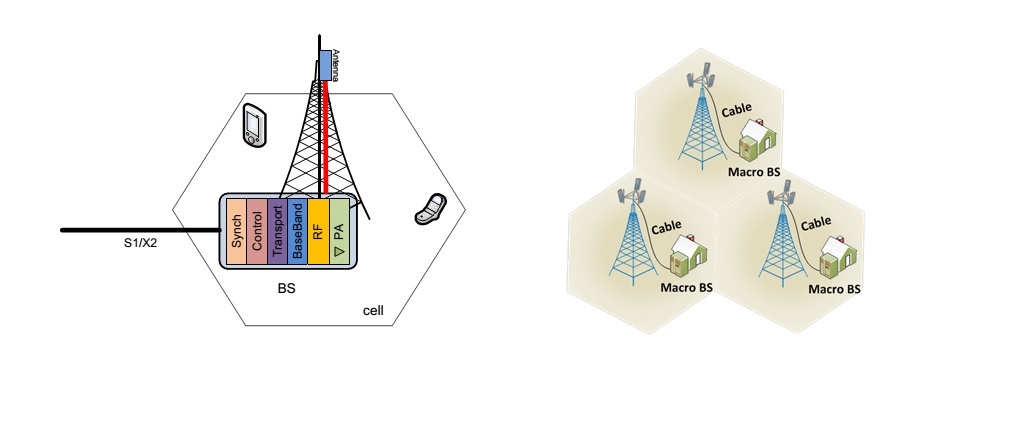
\includegraphics[scale=0.7]{./pic1/c11}
  \caption{ساختار سنتی ایستگاه پایه \cite{checko2015cloud}}
  \label{fig:c11}
\end{figure}
هر ایستگاه پایه دو نوع پردازش انجام می دهد : پردازش
رادیویی که توسط واحد رادیویی \LTRfootnote{RRH} انجام می شود و شامل پردازش
دیجیتالی، فیلترینگ فرکانسی، تقویت توان و ....میباشد و
پردازش باند پایه که توسط واحد باند پایه \LTRfootnote{BBU} که همان واحد کنترل است \LTRfootnote{CU} انجام شده و از جمله
مهمترین وظایف آن می توان به کدینگ، مدولاسیون و
تبدیل فوریه ی سریع اشاره کرد. در ساختار جدیدی که
تحت عنوان \lr{C-RAN}  معرفی خواهیم نمود نحوه ی ارتباط
پردازشگرهای رادیویی و باند پایه متحول شده و در نتیجه
مزایایی برای شبکه حاصل خواهد شد.در ادامه ، انواع ساختارها را بیان خواهد شد.

\subsection{پیش زمینه ها} 
\subsubsection{ساختار سنتی ایستگاه پایه }

در ساختارهای سنتی ایستگاه پایه، پردازش های رادیویی و باند پایه در
داخل ایستگاه پایه انجام می شد و مدول آنتن نیز در فاصله
ی چند متری از مدول رادیویی نصب شده و ارتباط آنها
توسط کابل کواکسیال برقرار می شد که همین امر سبب
افزایش تلفات در شبکه می باشد. این نوع ساختار در شکل
\ref{fig:c11} نشان داده شده است. همان گونه که مشاهده می کنید
ارتباط بین ایستگاههای پایه توسط ارتباط  $X_2$ و ارتباط بین
ایستگاه پایه و شبکه ی هسته توسط ارتباط $ S_1$ برقرار می
شود. این نوع ساختار در شبکه های \lr{1G} و \lr{2G} به کار گرفته
شده است 
\cite{checko2015cloud}.

%Figure \ref{fig:gull} shows a photograph of a gull.
\subsubsection{ ساختار ایستگاه پایه و واحد رادیویی}

\begin{figure}
  \centering
    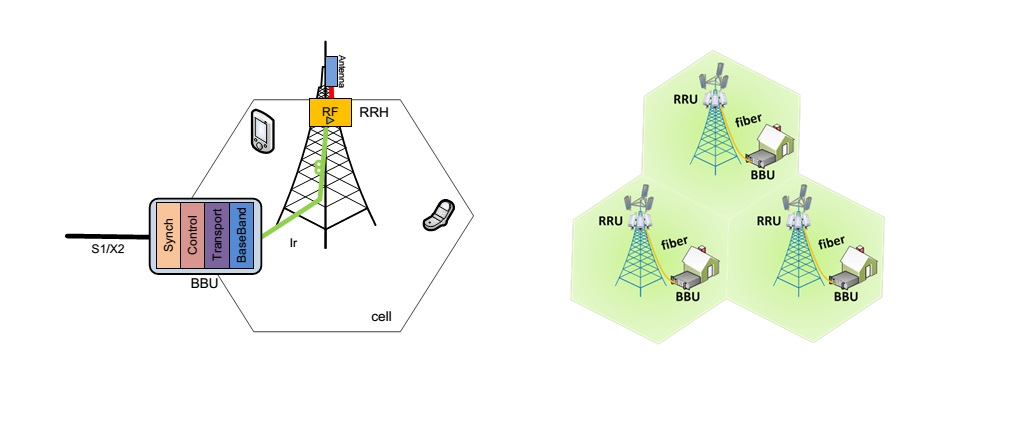
\includegraphics[scale=0.7]{./pic1/c22}
  \caption{ ساختار ایستگاه پایه و واحد رادیویی \cite{checko2015cloud}}
  \label{fig:c22}
\end{figure}
در این ساختار واحد رادیویی و واحد پردازشی سیگنال، از هم
مجزا شده و واحد رادیویی که تحت عنوان \lr{RRH} یا \lr{RRU}
نیز شناخته می شود، توسط فیبر نوری به واحد باند پایه یا \lr{BBU} اتصال می
یابد. همان طور که پیشتر بیان شد واحد رادیویی مسئولیت
انجام پردازش های دیجیتالی از جمله تبدیل انالوگ به
دیجیتال، دیجیتال به انالوگ، تقویت توان و فیلترینگ رابر عهده دارد، که تفکیک وظایف واحد پردازشی و واحد
رادیویی در این ساختار در شکل \ref{fig:c22} قابل مشاهده است. این
نوع ساختار برای شبکه های نسل سوم معرفی شده و امروزه
نیز بیشتر ایستگاههای پایه از همین ساختار بهره می گیرند.
از جمله ویژگی های بارز این ساختار امکان ایجاد فاصله
بین واحد رادیویی و پردازشی می باشد، که این فاصله به
دلیل تاخیر پردازشی و انتشاری نمی تواند از  $40$کیلومتر
فراتر رود. در این ساختار تجهیزات مرتبط با \lr{BBU} می
توانند به مکانی مناسبتر که قابل دسترس تر بوده و هزینه
ی اجاره و نگهداری کمتری را به اپراتورها تحمیل می
کنند منتقل شوند و واحد های رادیویی نیز در در پشت بام
ساختمان ها و مکان های مرتفع نصب می شوند که این
خود سبب کاهش هزینه های خنک سازی ادوات موجود
می شود. نحوه ی ارتباط بین \lr{RRH} و \lr{BBU} مشابه ساختار
سنتی بوده و \lr{RRH} ها نیز توسط معماری زنجیروار با هم
در ارتباطند.
\begin{figure}
  \centering
    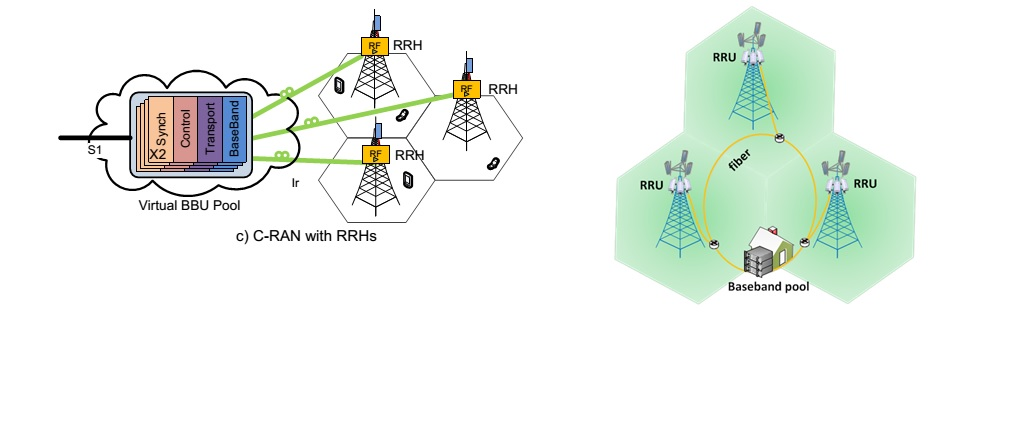
\includegraphics[scale=0.7]{./pic1/c33}
  \caption{ساختار  \lr{C-RAN} \cite{checko2015cloud}}
  \label{fig:c33}
\end{figure}
\subsection{تعریف مسئله}
\subsubsection{ساختار \lr{C-RAN}}
این ساختار جدید جزو یکی از ساختارهایی است که در \lr{5G} امکان استفاده را دارد.در این ساختار جدید در راستای بهینه سازی عملکرد \lr{BBU}
 ها در مواجهه باایستگاههای پایه پر ترافیک و کم ترافیک،
 \lr{BBU}ها به صورت یک مجموعه ی واحد تحت عنوان 
\lr{BBU Pool}
 در آمده اند که این مجموعه بین چندین سلول 
 به اشتراک گزارده شده و مطابق شکل زیر مجازی سازی
می شود. 
در توضیح بیشتر این ساختار می توان این گونه
عنوان کرد که \lr{BBU Pool} به عنوان یک خوشه ی مجازی
در نظر گرفته می شود که شامل پردازش گرهایی می باشد
که پردازش های باند پایه را انجام می دهند. ارتباط بین
  \lr{BBU}ها در ساختار های فعلی به شکل  $X_2$ برقرار می شود
که در این ساختار ارتباط بین خوشه ها از فرم جدید $X_2$
تحت عنوان  $X_2 +$برقرار می شود.
\newline
در شکل \ref{fig:c33} ساختار کلی شبکه ی  \lr{C-RAN} در سیستم های
\lr{ LTE}
 نمایش داده شده است. همان طور که در شکل قابل
مشاهده می باشد ساختار کلی شبکه  \lr{C-RAN} به دو بخش
 \lr{backhaul} و \lr{fronthaul} تقسیم بندی شده است. بخش
 \lr{fronthaul}شبکه به مرحله ی اتصال سایت های \lr{ RRH}به
 به \lr{BBU Pool} به اتصال \lr{backhaul} و بخش \lr{BBU Pool}
هسته ی شبکه ی سیار اطلاق می شود. همان گونه که قبلا
ذکر شد  \lr{ RRH}ها در نزدیکی انتن نصب شده و از طریق
لینک های انتقالی نوری با پهنای باند وسیع و تاخیر کم به
پردازشگرهای قوی در  \lr{BBU}متصل می شوند. توسط این
لینک های انتقالی است که سیگنال های دیجیتالی باند
پایه از نوع \lr{IQ} بین \lr{RRH} و \lr{BBU} انتقال می یابند \cite{checko2015cloud}.
\begin{figure}
  \centering
    \includegraphics[width=\textwidth]{./pic1/CRAN}
  \caption{ساختار شبکه ی \lr{C-RAN} \cite{checko2015cloud}}
  \label{fig:C-RAN}
\end{figure}
\section{مزایای شبکه ی \lr{C-RAN}}

در این بخش قصد داریم مزایای شبکه ی \lr{C-RAN} و هدف از استفاده ی آن در \lr{5G} را بیان کنیم.
\newline
در هر دو نوع سلولهای ماکرو و میکرو، می توان از ساختار \lr{C-RAN} بهره برد. در حالت ماکرو، متمرکز کردن \lr{BBU} ها به صورت \lr{BBU Pool}، منجر به استفاده ی بهینه از \lr{BBU} ها و کاهش هزینه ی ایستگاه پایه \LTRfootnote{base station} می شود. همچنین منجر به کاهش مصرف توان و فراهم کردن انعطاف پذیری بیشتر در شبکه و تطبیق آن با ترافیک غیر یکسان می شود. علاوه بر این، باعث تبدیل سیگنال تداخل به سیگنال مفید تبدیل می شود. در ادامه این مزایا به صورت گسترده تر بیان می گردد. \cite{checko2015cloud, namba2012colony}
\begin{figure}
  \centering
    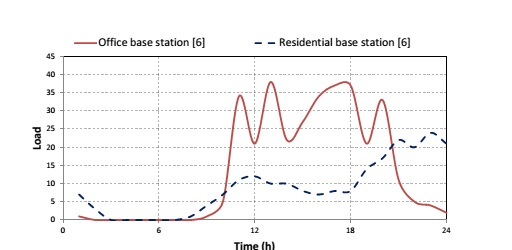
\includegraphics[width=\textwidth]{./pic1/c4}
  \caption{تغییرات حجم ترافیک در ایستگاههای پایه بنا به
مکان قرارگیری آنها \cite{checko2015cloud}}
  \label{fig:c4}
\end{figure}
\subsection{توانایی تطبیق پذیری با ترافیک غیر
یکنواخت }
کاربران شبکه های رادیویی در طول روز بین مناطق مختلف
(مسکونی و اداری) جابه جا شده و در نتیجه ترافیک هر
منطقه نیز بنا به نوع منطقه در طول ساعات شبانه روز متغیر
می باشد.
نمودار مربوط به این تغییرات در شکل \ref{fig:c4} قابل
مشاهده است. نکته ی قابل توجه برای اپراتور ها در این
بخش، هدر رفت توان پردازشی در اثر جا به جایی کابران می
باشد. بدین شکل که به طور مثال بعد از اتمام ساعات کاری
کاربران شبکه از مناطق اداری به مناطق مسکونی نقل مکان
می کنند حال انکه ایستگاههای پایه برای خدمات رسانی
در اوج ترافیک تعبیه شده و با کاهش تعداد کاربران در
حقیقت توان پردازشی هدر می ر ود. تحقیقات نشان داده
است که میزان پیک ترافیک شبکه حدود  $10$ برابر بیشتر
از ترافیک در ساعات غیر اوج می باشد و در هر سلول بنا
به نوع منطقه ساعات اوج ترافیک متغیر است. با توجه به
متغیر بودن ساعات اوج ترافیک در سلول های مختلف و
با استفاده از ویژگی شبکه های \lr{C-RAN} می توان راهکاری
ارائه نمود که از هدر رفت توان پردازشی جلوگیری شود.
در شبکه های \lr{C-RAN} پردازش های باند پایه مربوط به
چندین سلول به ابر منتقل شده که می توان از این ویژگی
برای افزایش نرخ بهره وری استفاده کرد.  \cite{checko2015cloud, namba2012colony} 
\subsection{صرفه جویی در هزینه و مصرف انرژی }
با بکارگیری شبکه های \lr{C-RAN} در مصرف انرژی و از این
رو در کاهش هزینه ها می توان صرفه جویی نمود.
هزینه
های صورت گرفته توسط اپراتورهای سیستم های مخابراتی
که تحت عنوان \lr{TCO} نیز شناخته می شود،به دو دسته
ی عمده تقسیم بندی می شود. هزینه های \lr{CAPEX} و
هزینه های \lr{OPEX}؛
که هزینه ی \lr{CAPEX} مربوط به ساخت شبکه که شامل طراحی و نصب سخت افزارها می باشد. هزینه ی \lr{OPEX} شامل هزینه های مربوط به راه اندازی و نگهداری وهمچنین
ارتقای شبکه ی مخابراتی می باشد. که \lr{C-RAN} منجر به کاهش هر دو هزینه می شود.
\subsection{سهولت در ارتقا دادن و نگهداری از شبکه}
با قرار گیری  \lr{ BBU} ها در داخل ابر به جای قرارگیری در
ایستگاه های پایه ی دور از هم امکانسهولت در ارتقا دادن و نگهداری از شبکه در صورت نیاز به مداخله ی نیروی انسانی
فراهم می شود، زیرا در این صورت به جای نظارت بر تمام
ایستگاههای پایه تنها تعداد مشخصی \lr{BBU pool} مد نظر
قرار می گیرند. هم چنین بروزرسانی \lr{CPU} در این حالت
تسریع شده و استفاده از تکنولوژی \lr{IT} به جای استفاده از
سخت افزارها هموارتر می شود.
\begin{figure}
  \centering
    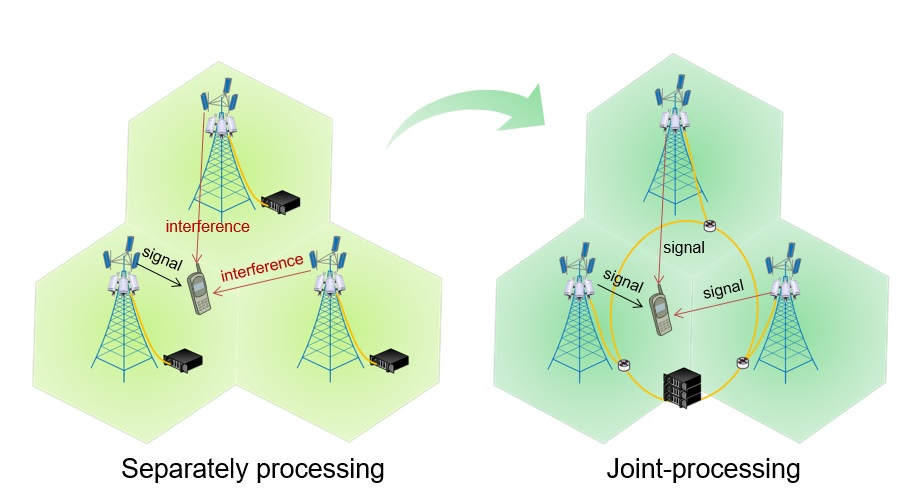
\includegraphics[width=\textwidth]{./pic1/c55}
  \caption{تداخل در \lr{LTE} و \lr{C-RAN} \cite{WinNT}}
  \label{fig:c55}
\end{figure}
\subsection{کاهش چشمگیر تداخل از طریق پردازش واحد باند پایه }
تداخل در شهرهای بزرگ یکی از چالشهای مهم محسوب می شود. \newline
همانطور که در شکل \ref{fig:c55} دیده می شود، در \lr{LTE} تداخل به صورت واضحی بر روی سیگنال مفید اثر می گذارد، حال در \lr{C-RAN} این مشکل به صورتی که در شکل دیده می شود برطرف شده و سیگنال تداخل تبدیل به سیگنال مفید می شود و از رابطه ی متقابل کانال \lr{TDD} \LTRfootnote{Time Division Duplexing} استفاده می گردد.

\subsection{افزایش توان و کاهش تاخیر}
در سالهای اخیر شبکه های نسل $4$  یا \lr{LTE} توسط \lr{ 3GPP}
استاندارد سازی شده و به مرور جایگزین سیستم های نسل $3$
 شده اند.
 
  شبکه های \lr{C-RAN} 
 با توجه به قابلیت هایی
که دارند در سیستم های نسل $4$ یعنی \lr{LTE} و \lr{LTE-A}
قابل پیاده سازی و بهره برداری بوده و مزایایی را برای این
سیستم ها به همراه خواهند داشت. برای توضیح بهتر نقش
   \lr {C-RAN} در افزایش توان عملیاتی نیاز هست که با تکنیک
هایی از قبیل  \lr{eICIC} و  \lr{CoMP} اشنا شده و سپس این
تکنیک ها را به ساختار \lr{C-RAN} تعمیم بدهیم.
همان طور که می دانید در سیستم های \lr{LTE} منابع به
صورت مشارکتی مورد استفاده قرار می گیرند. مسئولیت
تخصیص منابع در این شبکه ها به عهده ی زمانبندی 
به نام \lr{eNB} \LTRfootnote{eNode B} است که در ایستگاه پایه قرار دارد. نکته ی
قابل توجه دیگر استفاده از تکنیک \lr{OFDMA} می باشد که
زمانبند را قادر می سازد که منابع را به صورت دینامیکی
هم در حوزه ی زمان و هم در حوزه ی فرکانس به کاربران
مختلف تخصیص دهد.
با توجه به این که در سیستمهای \lr{ LTE} عموما پارامتر استفاده
ی مجدد از فرکانس برای تمامی سلول ها یک در نظر
گرفته می شود، در نتیجه تداخل بین سلول های مجاور
به شدت افزایش می یابد. برای رفع این مشکل دو روش
عمده مطرح می شود: روش اول کاهش تداخل و روش دوم
استفاده ی سازنده از تداخل. برای پیاده سازی روش اول
از تکنیک \lr{ICIC} یا \lr{eICIC} استفاده می شود و برای روش
دوم عمدتا از تکنیک \lr{CoMP} بهره می گیرند که توضیح
نحوه ی عملکرد این تکنیک ها در مقاله ها به طور کامل
بررسی شده است. در رابطه با کاهش تاخیر نیز می توان
این گونه عنوان نمود که با قرار گرفتن \lr{ BBU} ها در مجاورت
هم در ابر مدت زمان لازم برای انجام عمل \lr{hand off} بین
ایستگاههای پایه کاهش می یابد. زیرا عمل\lr{hand off} در
این حالت به جای ایستگاههای پایه در \lr{ BBU} ها صورت
می گیرد
\section{چالشها و مشکلات در برخورد با ساختار \lr{C-RAN} }

\subsection{دو چالش مهم مربوط به \lr{fronthaul}}
 \begin{figure}
  \centering
    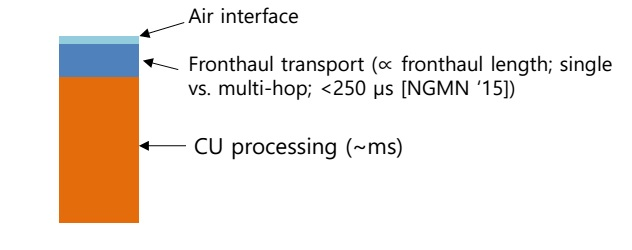
\includegraphics[scale=0.7]{./pic1/c6}
  \caption{محدودیت در اثر تاخیر \cite{simeoneConf}  }
  \label{fig:c6}
\end{figure}
یکی از مشکلات پیش روی ساختار \lr{C-RAN} در قسمت \lr{fronthaul} به شرح زیر است.
\begin{itemize}
\item
 محدودیت ظرفیت که
 به دو دلیل ایجاد می گردد که در ادامه ذکر شده است \cite{simeoneConf}.
 \begin{itemize}
 \item
 نمونه برداری و کوانتیزاسیون اسکالر
 \item
 تداخل رادیویی به صورت عمومی
 \end{itemize}
  
 \item 
  محدودیت در اثر تاخیر که
   به سه دلیل ایجاد می شود که در ادامه ذکر شده است \cite{simeoneConf}.
  \begin{itemize}
 \item
 تداخل هوا
 \item
 انتقال سیگنال در قسمت \lr{fronthaul}
 \item
 پردازش واحد کنترل
 \end{itemize}
   انتقال سیگنال در قسمت \lr{fronthaul} و پردازش واحد کنتذل به نوع انتقال \lr{fronthaul} بستگی دارد (بسیم یا انتقال با سیم) 
\end{itemize}
با استفاده ازمخابرات فیبر نوری این مشکلات تا مقدار زیادی حل خواهد شد. 
\subsection{نحوه ی مشارکت \lr{BBU} ها نحوه ی اتصال
و خوشه بندی}

همکاری بین ایستگاههای پایه بایستی به گونه ای باشد
که از نظر زمانبندی و بررسی اطلاعات بازخورد کانالها
به منظور مدیریت تداخل و همچنین سازگاری باتکنیک
   \lr{CoMP}مورد بررسی قرار گرفته باشد.
تکنیک هایی که برای اتصال \lr{BBU}ها مورد استفاده قرار
می گیرند بایستی از نظر امنیت، قابلیت اطمینان، پشتیبانی
از پهنای باند وسیع ،تاخیر کم و ... استاندارد های لازم را
براورده ساخته و نسبت به ساختار سنتی عملکرد بهتری را
از خود نشان دهند.
\subsection{نیاز به پهنای باند وسیعتر و تاخیر
دقیق و کمتر}
در ساختار شبکه ی \lr{C-RAN} اطلاعات به صورت \lr{ IQ} بین
 \lr{RRH} و  \lr{BBU} ها انتقال می یابند. طبق استانداردهایی
که برای این شبکه تعریف شده است، انتظار می رود که
هر \lr{BBU pool} قابلیت خدمات دهی به $100-1000$
ایستگاه پایه را دارا باشد. بنابراین با توجه به پهنای
باند مورد نیاز برای ارسال اطلاعات به صورت \lr{ IQ} حجم
اطلاعاتی زیادی توسط لینک های نوری به سمت \lr{BBU pool}
  ها سرازیر خواهد شد و پهنای باند بالایی مورد نیاز
است.علاوه بر نیاز به پهنای باند بالا شبکه ی انتقال ما
بایستی نیاز به جیتر و تاخیر دقیق در شبکه را برآورده کند،
که در ادامه برخی از این قیود لازم آورده شده است.
\begin{itemize}
\item
دقت زمانی لازم برای همکاری بین ایستگاههای پایه
بایستی در حدود $ 0.5 \mu sec$ باشد که مهم ترین شرط
این مبحث محسوب می شود.
\item
صرف نظر از تاخیر حاصل از طول
کابل تاخیر حاصل از رفت و برگشت اطلاعات کاربران
نبایستی از حدود $ 5 \mu sec$ بیشتر باشد
\item
فاصله ی بین \lr{RRH} و \lr{BBU} ها بایستی از حد 
 $ 20 - 40 km$تجاوز نکند و تاخیر حاصل از پردازش زیر
 فریم ها در لینک های ارتباطی بین  \lr{RRH} و \lr{BBU} نیز
بایستی از $1ms$ کمتر باشد
\end{itemize}
\subsection{محدودیت ظرفیت در \lr{backhaul}}
همچنین محدودیت ظرفیت در \lr{backhaul} منجر به محدود کردن عملکرد انتقال در حالت مشارکت چند نقطه ای  در  \lr {C-RAN} می گردد. 
\subsection{نیاز به شبکه های انتقال ازران}
برای انتقال اطلاعات بین \lr{RRH} و \lr{BBU} از فیبر نوری
استفاده می شود. فیبر نوری به دلیل سرعت در انتقال
اطلاعات تلفات کم و قابلیت انتقال حجم بالایی از
اطلاعات گزینه ی مناسبی برای شبکه های \lr{C-RAN} به
حساب می اید. با وجود محاسن گفته شده گران بودن و
عدم دسترسی تمام اپراتورها به فیبر نوری از جمله مشکلاتی
است که بایستی قبل از پیاده سازی شبکه های \lr{C-RAN} بدان
پرداخته شود. \cite{MA}
\section{شبکه های دسترسی رادیویی ابری نا متجانس (\lr{H-CRAN})}
برای غلبه بر چالش های شبکه های \lr{C-RAN} با محدودیت های \lr{fronthaul} ، شبکه های دسترسی ابری نامتحانس (\lr{H-CRAN}) معرفی گردید\cite{ fogComputing, heterogeneous, fogEdge}.
\begin{figure}
  \centering
    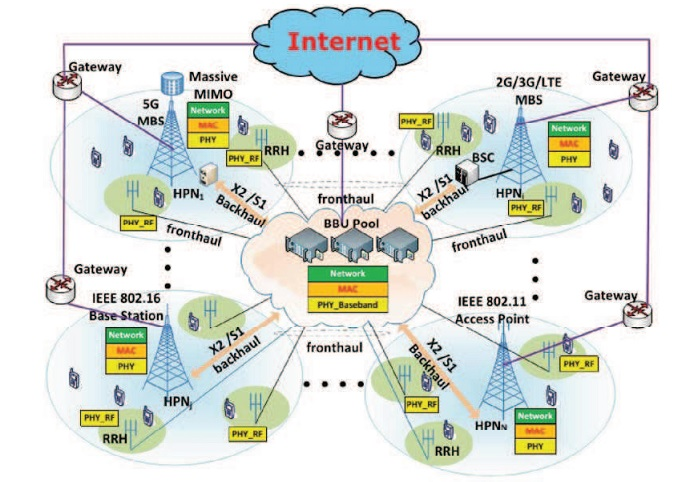
\includegraphics[scale = 0.8]{./pic1/hc}
  \caption{ ساختار شبکه های دسترسی ابری نامتحانس \cite{heterogeneous}  }
  \label{fig:hc}
\end{figure}

\subsection{ساختار شبکه ی \lr{H-CRAN}}
کاربر و صفحه ی کنترلگر در چنین شبکه هایی از هم مجزا می باشند. که در این شبکه ها ، نودهای توان بالا   \LTRfootnote{High Power Node}\lr{HPN} ، عمدتا برای فراهم کردن پوشش بدون درز و اجرای عملکرد صفحه کنترل می باشد. در حالی که \lr{RRH} ها برای فراهم نمودن سرعت بالای نرخ داده برای انتقال بسته در ترافیک قرار گرفته اند. \lr{HPN} ها از طریق لینکهای \lr{backhaul}  به \lr{BBU Pool} متصلند ( برای هماهنگ کردن تداخل ).\newline
ساختار این شبکه شبیه به ساختار \lr{C-RAN} می باشد . همانطور که در شکل \eqref{fig:hc} نشان داده شده است ، تعداد زیادی \lr{RRH} ، همراه با انرژی مصرفی کم در ساختار \lr{H-CRAN} ، با یکدیگر در \lr{BBU Pool} مرکزی ، همکاری می کنند تا گین مشترک بالایی بدست آورند.   تنها ، فرکانس رادیویی جلو ،(\lr{RF}) و عملکردهای پردازشی  ساده ، در \lr{RRH} ، صورت می گیرد ، در حالی که پردازشهای مهم دیگر ، در \lr{BBU Pool} انجام می گیرد. همچنین تنها بخشی از عملکردها در لایه ی \lr{PHY} در \lr{RRH} به مشارکت می انجامد که این مدل در شکل \eqref{fig:hc} نشان داده شده است.\newline
اگرچه ، برخلاف \lr{C-RAN} ، \lr{BBU Pool} در \lr{H-CRAN} ، به \lr{HPN} ها متصلند که این، برای کاهش تداخل متقابل بین \lr{RRH} ها و \lr{HPN} ها از طریق محاسبات ابری متمرکز بر اساس تکنیکهای پردازشی مشترک می باشد. همچنین ، داده و واسط کنترل ، بین \lr{BBU Pool} و \lr{HPN} های $S_1$ و $X_2$ شناخته شده اند که تعریف آنها بر اساس تعریف استاندارد \lr{3G} ایجاد شده است.\newline
همانطور که سرویسهای صدا ، می توانند به صورت بهینه در طول مد سوییچ بسته در \lr{4G} فراهم گردند ، \lr{H-CRAN} می تواند به طور همزمان سرویس صدا و داده را پشتیبانی کند. سرویس صدا مرجح به اداره از طریق \lr{HPN} ها می باشد ، در حالی که ترافیک بسته ی پر داده ، بیشتر توسط \lr{RRH} اداره می گردد. 
در مقایسه با ساختار \lr{C-RAN} ،ساختار \lr{H-CRAN} ، نیازهای \lr{fronthaul} را بوسیله ی مشارکت \lr{HPN} ها برطرف می سازد. با توجه به حضور \lr{HPN} ها ،سیگنالهای کنترلی و سمبلهای داده در \lr{H-CRAN} جدا از هم می باشند. تمام کنترل کننده های سیگنال و سیستم هایی که اطلاعات را ارسال می نمایند ، توسط \lr{HPN} ها به \lr{UE} ، منتقل می گردد که منجر به سادگی در ظرفیت و در محدودیت تاخیر زمان در لینکهای \lr{fronthaul } بین \lr{RRH} ها و \lr{BBU Pool}  می گردد و منجر به صرفه جویی در مصرف انرژی می گردد. همچنین ، برخی از ترافیک های شدید و ناگهانی \LTRfootnote{Burst Traffic} و یا سرویس پیام همراه با مقدار داده ی کم ، می تواند به صورت بهینه توسط \lr{HPN} ها پشتیبانی گردد. مکانیزم کنترل بین ارتباط داشتن و نبود ارتباط ، توسط \lr{H-CRAN} پشتیبانی می گردد که منجر به حفظ کردن مقدار قابل توجهی \lr{Overhead} در رادیو بوسیله ی مکانیزم ارتباط جهت دار خالص می گردد. در \lr{RRH} ، تکنولوژی های مختلف انتقال در لایه ی \lr{PHY} ، قابل استفاده برای بهبود نرخ انتقال (همانند موج میلیمتری و نور مرئی) می گردد. در \lr{HPN}ها، \lr{MIMO}\LTRfootnote{Multiple Input Multiple Output}، یکی از راه های افزایش پوشش در بهبود ظرفیت می باشد.

\subsection{چالشهای پیش روی \lr{H-CRAN}}
متاسفانه ، \lr{H-CRAN} در عمل دچار چالشهایی است.
\begin{itemize}
\item
 اولین چالش به این دلیل است که با معروفتر شدن موقعیتهایی که بر اساس کاربردهای اجتماعی است ، داده های ترافیکی در طول مسیر  \lr{fronthaul} از \lr{RRH} به \lr{BBU Pool}، با افزایش موج زیادی از داده های زائد همراه است که منجر به بدتر شدن محدودیت \lr{fronthaul} می گردد.
\item
همچنین \lr{H-CRAN} ، از تمامی فواید پردازشی و ظرفیت ذخیره در ابزارهای پردازشی و الکترونیکی همانند \lr{RRH} و تلفن های هوشمند (\lr{UE}) ،که راه های رسیدن به موفقیت در این ساختار است ، استفاده نمی کند .
\item
همچنین ، اپراتورها ،نیاز به استقرار تعداد زیادی \lr{RRH} و \lr{HPN} ثابت در \lr{H-CRAN} ، می باشند تا به ماکسیمم ظرفیت دسترسی پیدا کنند. ولی در زمانهایی مه ترافیک زیاد نیست ، منجر به اتلاف شدیدی می شود. 
\end{itemize}
\section{\lr{C-RAN}و \lr{H-CRAN} }

\subsection{تفاوت و شباهت های این دو ساختار}
  تفاوت عمده ی بین این دو ساختار در این است که در \lr{H-CRAN} ، عملگر کنترل مرکزی از \lr{BBU Pool} به \lr{HPN} منتقل گردیده است. \cite{fogComputing}
 \newline
در هر دو ساختار، عملگرهای \lr{CRSP} \LTRfootnote{Collaboration Radio Signal Processing} و ذخیره سازی اطلاعات در سرور ابر مرکزی ، صورت می گیرد که نیاز به تعداد زیادی دستگاه های فرستنده (موبایل) و انتقال داده به سرعت کافی از طریق \lr{BBU Pool} می باشد.
\subsection{مشکلات پیش روی این دو ساختار}
مهمترین مشکلات این دو ساختار ، تاخیر انتقال زیاد و سنگینی حمل اطلاعات بر روی \lr{fronthaul} می باشد.روش ساده یرای حل این مشکل :
\begin{itemize}
\item
جلوگیری از انتقال تمام داده ها به \lr{BBU Pool} شویم و بخشی از پردازش اطلاعات را در \lr{RRH} های محلی و همچنین وسایل الکترونیکی هوشمند انجام دهیم.
\item
جلوگیری کنیم از اینکه همه ی ترافیک به طور مستقیم از سرور ابر متمرکز منتقل شود، برخی از ترافیک محلی باید از ذخیره  \lr{RRH} های مجاور تحویل گردد.
\end{itemize}
\section{ارائه ی پیشنهاد سیستم جایگزین (\lr{F-RAN})}
برای حل کردن مشکلات \lr{H-CRAN} و \lr{C-RAN}، نیاز به معرفی ساختار جدید دیگری می باشیم که آن را \lr{F-RAN} می نامیم.
\lr{F-RAN} تمام ویژگی های مثبت محاسبات ابری و شبکه های نامتجانس و محاسبات مهی را همزمان در بر می گیرد.
محاسبات مهی ، اصطلاحی برای جایگزین کردن محاسبات ابری است که مقدار قابل توجهی از ذخیره سازی ، ارتباطات ، کنترل کردن ، اندازه گیری و مدیریت را در لبه ی شبکه انجام می دهد (نه در کانال و ابر مرکزی) \cite{fogComputing, fogEdge,fog12}.
\begin{figure}
  \centering
    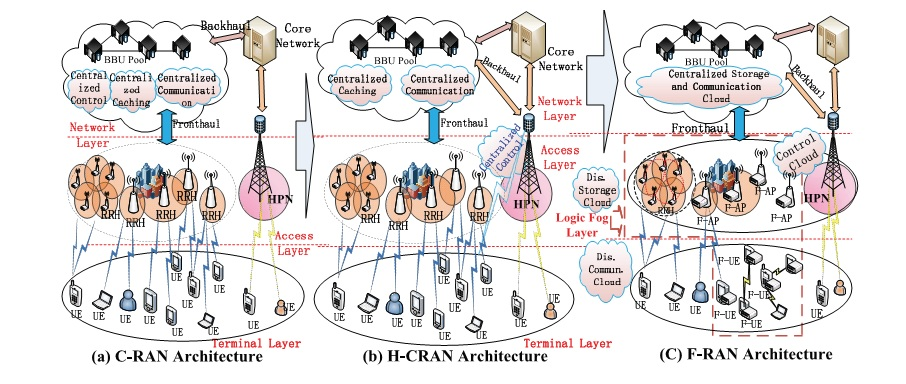
\includegraphics[scale = 0.7]{./pic1/fhc}
  \caption{ سیر تحولات شبکه های رادیویی ابری \cite{fogComputing}}
  \label{fig:fhc}
\end{figure}
\subsection{ساختار سیستمهای   \lr{F-RAN}}
 سیستمهای \lr{F-RAN} تحولی از سیستمهای \lr{C-RAN} می باشد که در شکل \eqref{fig:fhc} نشان داده شده است. برخی از ارتباطات توزیع شده و عملکردهای ذخیره سازی در منطق لایه ی مه قرار دارد. همچنین چهار نوع ارتباطات ابری تعریف شده است.
  \begin{figure}
  \centering
    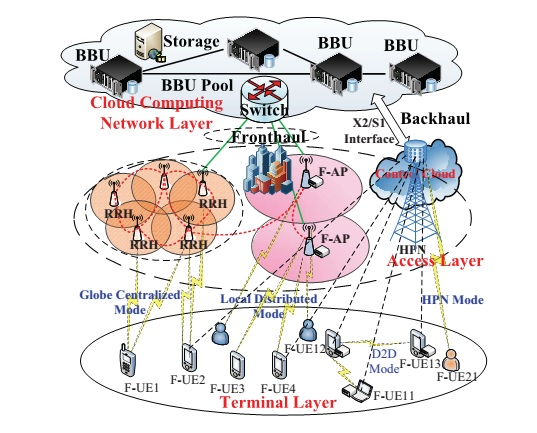
\includegraphics[scale =0.7]{./pic1/fr}
  \caption{ مدل سیستم \lr{F-RAN} \cite{fogComputing} }
  \label{fig:fr}
\end{figure}
 \begin{itemize}
 \item
 ابر ذخیره گر و ارتباطات مرکزی جامع :
 که همانند ابر مرکزی \lr{C-RAN} می باشد
 \item
 ابر کنترل گر مرکزی :که برای تکمیل عملکردهای کنترلی  می باشد و در \lr{HPN} ها قرار دارد
 \item
 ابر ارتباطات منطقی توزیع شده که در برنامه های محاسبات مهی و ابزار های این محاسبات قرار دارد.
 \item
  ابر ذخیره گر منطق توزیع شده:
  که همانند قبل در \lr{F-RAN} قرار دارد.
 \end{itemize}
 در این ساختار ، برای کاهش تاخیر ناشی از انتقال داده ها به ابر مرکزی ، ساختار های \lr{RRH} را دارای حافظه قرار می دهیم که برای ارتباطات محلی، به جای اینکه پردازش ها در \lr{BBU Pool} صورت بگیرد، بدون نیاز به انتقال به ابر مرکزی، درون \lr{RRH} ها انجام پذیرد. 
 %%%%%%%%%%%%%%%%%%%%%%%5
 %%%%%%%%%%%%%%%%%%%%%%%
 \section{برخی از کاربردهای شبکه ی \lr{C-RAN}  }

\subsection{ تخصیص منابع مبتنی بر مدولاسیون \lr{OFDM}}
هدف از متد ارائه شده در برخی مقالات را می توان تخصیص
منابع بین سلول ها با در نظر گرفتن تداخل بین سلول و هم
چنین کاهش تعداد \lr{BBU} های فعال عنوان کرد. نحوه ی
تخصیص به  ۲بخش تقسیم شده و به طور جداگانه بررسی
شده است. بخش اول و اصلی تخصیص منابع بین ناحیه
های لبه سلول ها می باشد که بایستی تداخل در نظر گرفته
شده و بدان منظور از روش \lr{graph coloring} استفاده شده
است و بخش دوم تخصیص منابع بین ناحیه های مرکزی
می باشد که بنا به تخصیص های صورت گرفته در بخش
اول انجام می شود. در ادامه عملکرد متد ارائه شده برای
تخصیص منابع مبتنی بر شبکه \lr{C-RAN} بررسی شده و مورد
ارزیابی قرار می گیرد.
در سناریو مورد نظر شبکه ای شامل  ۹سلول در نظر گرفته
و پهنای باندی که که به هر \lr{BBU} تخصیص داده می
شود را برابر $ B = 20MHZ$ در نظر گرفته و تابع توزیع
احتمال ترافیک شبکه را نیز گوسی در نظر می گیریم. دو
پارامتر $\sigma_ck$ و $\sigma_ek$به ترتیب نشانگر پهنای باند مورد نیاز ناحیه
ی لبه و ناحیه ی مرکزی سلول  می باشند. پهنای باند
مورد نیاز به صورت مستقل و یکسان بین تمام سلولها توزیع
شده است .\cite{graph}
\begin{figure}
  \centering
    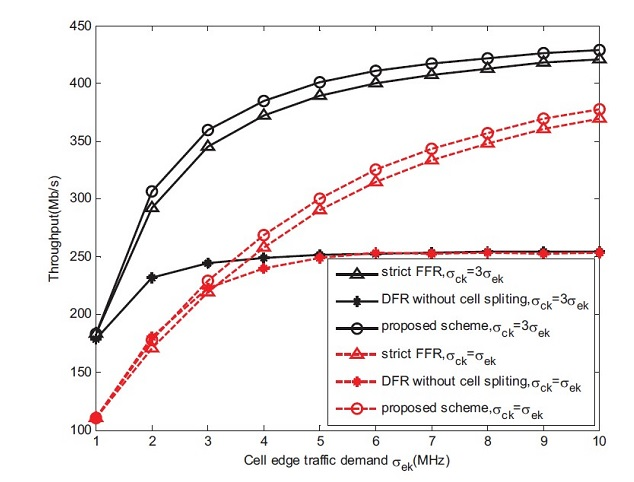
\includegraphics[scale =0.7]{./pic1/cr}
  \caption{ توان عملیاتی تمام کاربران سلول \cite{graph} }
  \label{fig:cr}
\end{figure}
در شکل \eqref{fig:cr}  توان عملیاتی تمام کاربران سلول چه کاربران
نواحی مرکزی یا لبه مورد بررسی قرار گرفته است. در این
 دو دسته نمودار حاصل می
نمودار با انتخاب  $\frac{\sigma_ck}{\sigma_ek} = \frac{1}{3}$ 
شود که وابستگی عملکرد به تغییرات ترافیک را نشان می
دهند. در نمودار های مذکور متد جدیدی تحت عنوان \lr{DFR} بدون تجزیه ی سلول نیز مشاهده می شود که نحوه
ی تخصیص مطابق روش ارایه شده ما می باشد با این
تفاوت که نواحی لبه و مرکزی تفکیک نشده و کل سلول
واحد در نظر گرفته شده است. با هر دو انتخاب ممکن برای
نسبت ترافیک ها می توان مشاهده کرد که متد ما عملکرد
بهتری را از خود به نمایش می گذارد. متد   \lr{DFR} بدون
تفکیک سلول نیز بدترین عملکرد را از خود نشان می دهد
زیرا نمی تواند به طور بهینه از منابع استفاده کند
در شکل های \eqref{fig:7} و \eqref{fig:8} نیز عملکرد بهره وری انرژی هر ۳
متد مورد نقد و بررسی قرار گرفته است. شایان ذکر است
که میزان بهره وری انرژی به نسبت توان عملیاتی تمام
کاربران به توان تمام \lr{BBU} های فعال اطلاق می شود. با
توجه به نمودار ها بدترین عملکرد متعلق به روش \lr{FFR}
معمول می باشد زیرا به ازای هر سلول از یک  \lr{BBU}مجزا
استفاده می شود.
نکته ی قابل توجه در این نمودار عملکرد
بهتر متد \lr{DFR} بدون تفکیک سلول نسبت به متد ارائه شده
است .علت این امر نیز استفاده از  \lr{BBU}ها ی کمتر از
$\frac{M}{3}$
می باشد. هر چند اگر ما تعداد کمتری کاربر در هر سلول داشته
باشیم و حجم ترافیکی کاهش یابد، نتایج حاصل از متد ارایه
شده از متد \lr{DFR} بدون تفکیک سلول پیشی گرفته و بهترین
عملکرد را از خود نشان می دهد که نتایج مذکور در شکل
  \eqref{fig:8}
   قابل مشاهده است. در این نمودار فرض
\begin{equation*}
\sigma_e k = \sigma_c k
\end{equation*}  
 رعایت شده و میزان $\sigma_ek$ بین  0.2 و 2 انتخاب می شود
با مفروضات انجام شده تعداد \lr{BBU} های فعال در هر دو
متد یکسان شده و چون توان عملیاتی کاربران در متد ارائه
شده بهتر است پس متد مذکور در این نمودار نیز بهترین
عملکرد را نسبت به  2متد دیگر از خود نشان می دهد.  
\begin{figure}
  \centering
    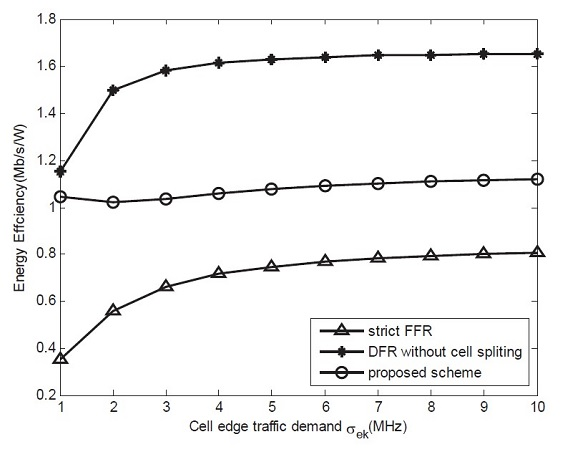
\includegraphics[scale=0.7]{./pic1/7}
  \caption{ بهره وری انرژی در حضور ترافیک معمول \cite{graph}  }
  \label{fig:7}
\end{figure}

\begin{figure}
  \centering
    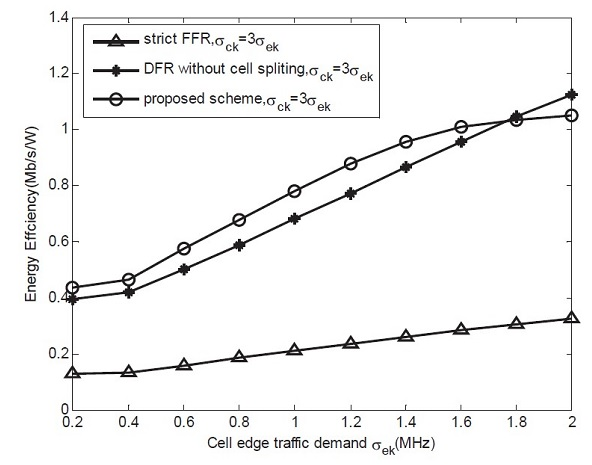
\includegraphics[scale=0.7]{./pic1/8}
  \caption{  بهره وری انرژی در حضور ترافیک محدود \cite{graph} }
  \label{fig:8}
\end{figure}
\section{تخصیص توان و خوشه بندی شبکه های رادیویی ابری}
برای کاهش پیچیدگی این نوع شبکه ها ، می توان از تکنیک های خوشه بندی در طراحی و چینش\lr{RRH} ها استفاده کرد. برای بهبود بازدهی انرژی و توان نیز می توان تخصیص توان و خوشه بندی شبکه های رادیویی ابری را همزمان با هم انجام داد. 
که این مبحث یکی از بحث های داغ در شبکه های رادیوی ابری می باشد که با روش های بهینه سازی به طور همزمان به تخصیص توان و بدست آوردن تعداد خوشه ها خواهیم رسید .
حتی برای خوشه بندی به طور تنها نیز می توان از روش \lr{K Means} استفاده کرد . در شکل \ref{fig:88} نموداری از نسبت خطا به تعداد  \lr{RRH} در هر خوشه رسم شده است. 
\begin{figure}
  \centering
    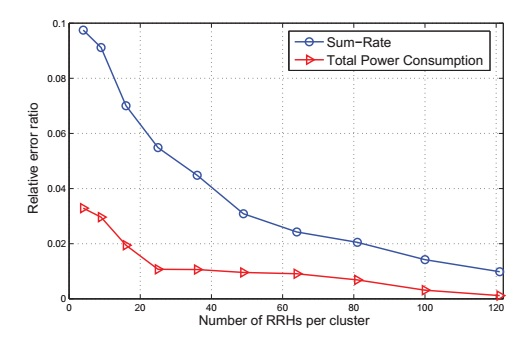
\includegraphics[scale=0.7]{./pic1/88}
  \caption{  نسبت خطا به تعداد \lr{RRH} در هر خوشه \cite{graph}  }
  \label{fig:88}
\end{figure}
\section{نتیجه گیری}
در این فصل، نسل پنجم مخابرات یعنی \lr{5G} و ساختار جدید \lr{C-RAN} که مورد توجه در این نسل مخابرات است ،مورد بررسی قرار گرفته شده و مزایا و چالش های پیش روی آن به طور مختصری بیان کرده ایم . همچنین ساختار های جدیدی که ساختارهای تعمیم یافته ی \lr{C-RAN}می باشد را مورد بررسی قرار داده ایم.این ساختارهای جدید قابلیت کاهش هزینه های ساخت و بهره
برداری از شبکه و هم چنین بهبود کارایی سیستم از لحاظ
پوشش دهی و تحرک پذیری را دارا می باشد و شاید بتوان
افزایش بهره ی انرژی را جزو مهمترین مزایای این ساختار
عنوان کرد. 


\section{خلاصه ای از فصلهای آتی}
در فصلهای بعدی، مدل سیستم ساختار \lr{C-RAN} مورد بررسی قرار می گیرد.
در فصل 2 به کارهای گذاشته و مدل سیستمهای گذشته در لینک فروسو و فراسو می پردازیم و مفهومی به نام بازدهی انرژی\LTRfootnote{Energy efficiency}
را بیان می کنیم و هدفمان در این فصول بیشینه سازی مجموع نرخ های قابل دسترس و بیشینه سازی بازدهی انرژی می باشد.
در فصل سوم به بررسی مدل سیستم جدیدی می پردازیم که نسبت کارهای قبلی تغییرات اندکی کرده است و در فصل چهارم نیز مدل سیستمی با تغییرات بیشتری را در نظر داریم و در نهایت در فصل پنجم به نتیجه گیری تمام فصل ها پرداخته می شود.






\newpage
{
\onehalfspacing
\bibliographystyle{acm-fa}
\bibliography{MyReferences}
}

 

\end{document}
